\chapter{Related Work\label{cha:chapter5}}

\hspace*{1em}
\begin{figure}[b!]
    \centering
    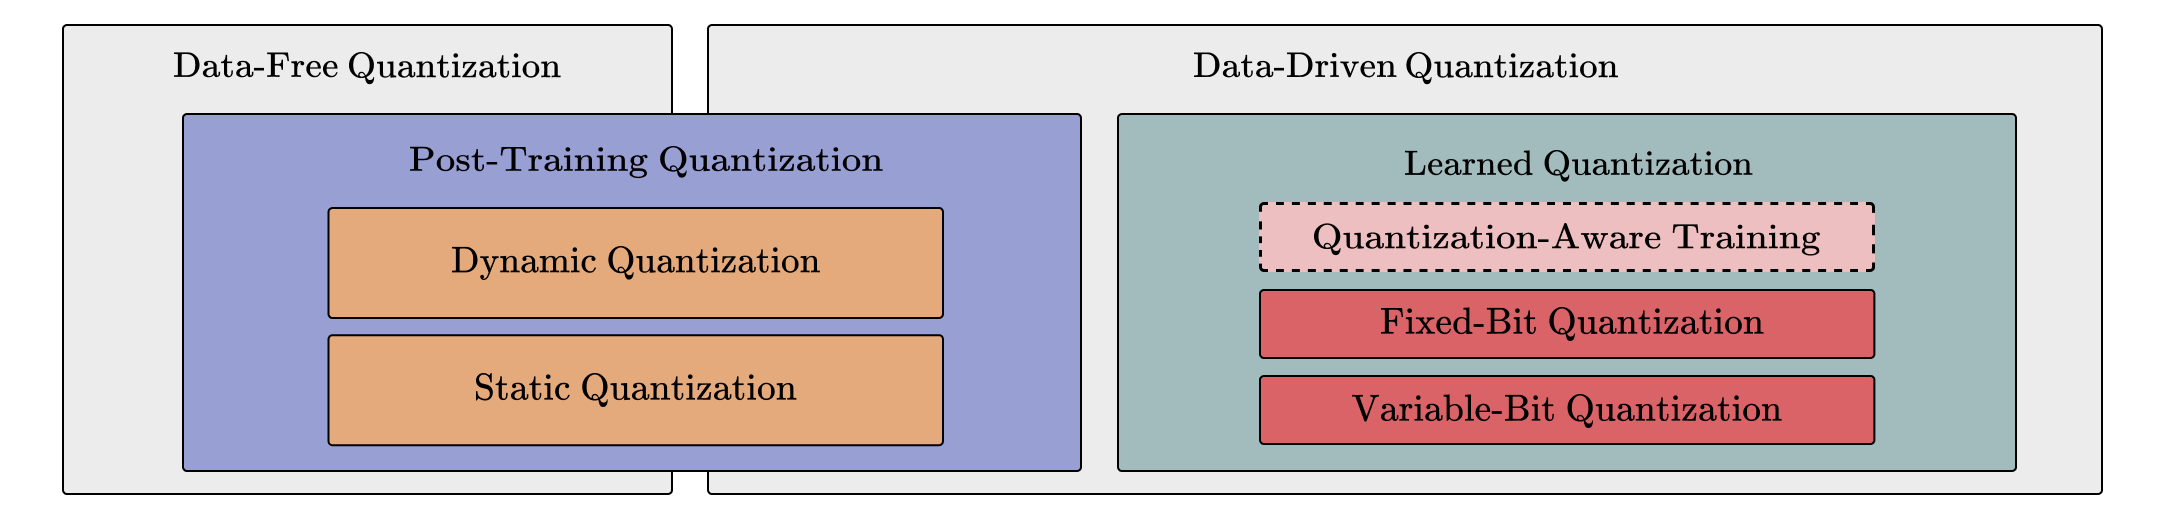
\includegraphics[width=14cm]{related_work.png}
    \caption{ Learned quantization in a broad context.}
    \label{fig:related_work}
  \end{figure}
  
The hyperparameter space of deep neural networks is so vast
that classifying research in the field of learned quantization into rigid groups
is inherently challenging.
Nevertheless, we aim to outline a rough distinction
between different approaches by emphasizing their most apparent aspects,
after first establishing the position of learned quantization within the broader field of quantization.

\textbf{Data-Free vs. Data-Driven Quantization.}
As discussed in \cref{cha:chapter2}, 
data-free quantization relies solely on the intrinsic properties of ML models, 
such as weight distribution statistics, to determine quantization parameters \cite{DBLP:conf/iccv/NagelBBW19}. 
In contrast, data-driven quantization uses the original training data to fine-tune the model to the quantization strategy \cite{Edouard2022SPIQ}. 
Although learned quantization does not strictly align with the definition of a fine-tuning process, 
it incorporates the full training pipeline, jointly optimizing both the model and the quantization parameters. 
This characteristic makes it inherently data-driven. 
Thus, we regard learned quantization as a distinct subcategory within data-driven quantization approaches.

\textbf{PTQ vs. QAT.}
Although PTQ and QAT are often presented as contrasting approaches in the literature, 
they differ fundamentally in their nature.
PTQ refers to a collection of techniques applied after a model has been trained to quantize its parameters, 
whereas QAT is a specific training process 
where the model is trained while incorporating quantization 
constraints throughout the training phase.
Thus, we classify QAT as part of learned quantization, 
while PTQ is considered a distinct approach, 
situated between data-free and data-driven quantization methods, 
as PTQ \cite{DBLP:conf/icmcs/ZhuZL18} can fall into either category depending on the parameters being quantized.
When only weights are quantized, the process is data-free, 
as weights can be quantized without relying on input data. 
When activations are included, the process becomes data-driven,
since activation quantization requires input data for calibration.

\textbf{Static vs. Dynamic Quantization.} 
Static quantization is an offline method that quantizes weights and activations before inference, 
whereas dynamic quantization is applied on-the-fly during inference. 
Both static and dynamic quantization methods are post-training approaches. 
In the context of learned quantization, 
static quantization might refer to a fixed quantization scheme, 
and dynamic quantization  — to a scheme 
that depends on trainable quantizers.
However, these terms are not commonly used this way in the literature.
Therefore, we consider static and dynamic quantization separately from learned quantization. 

Having established the broader context of quantization, 
we will now attempt to classify the various approaches within learned quantization itself.

\textbf{Fixed-Bit vs. Variable-Bit.} 
Learned quantization schemes can be roughly divided into two broader groups. 
The first group involves quantization schemes that use a fixed target bit size, 
while the second group aims to learn or effectively determine the lowest feasible bit size. 
This distinction is not widely discussed in the literature, 
but we view it as a recognizable pattern. 
For example, LQ-Nets \cite{DBLP:conf/eccv/ZhangYYH18} compute binary encodings of model parameters using a predefined bit size, 
whereas LSQ \cite{DBLP:conf/iclr/EsserMBAM20} learns step sizes in a way that can adaptively reduce bit-width requirements.

\textbf{Quantization Target.} NNs offer multiple opportunities for applying quantization.
While some learned quantization approaches focus exclusively on model weights \cite{polino2018modelcompression, ott2016rnn, courbariaux2015binaryconnect, DBLP:journals/pnas/EsserMACAABMMBN16},
others extend the target to include activations \cite{krishnamoorthi2018quantizing,hubara2016qnn,rastegari2016xnor,Edouard2022SPIQ,DBLP:conf/eccv/ZhangYYH18}
and even gradients \cite{DBLP:journals/corr/LinCMB15,DBLP:conf/icml/Zhang0KALZ17}. As notable examples,
DoReFa-Net \cite{shuchang2016dorafenet} quantizes all three with arbitrary bit widths, 
whereas Quantized Neural Networks \cite{hubara2016qnn} constrain weights and activations to either 
\( -1 \) or \( +1 \), and quantize gradients to \( 6 \) bits.

\textbf{Quantization Precision.}
The target lower bit precision, and whether it is adjustable, 
varies between methods — ranging from rigid constraints to only a few values, 
to the flexibility of setting the desired bit width. 
For instance, BinaryNet \cite{DBLP:conf/nips/HubaraCSEB16} and XNOR-Net \cite{rastegari2016xnor} 
represent extreme cases of quantization, 
where weights and activations are binarized. 
Ternary Weight Networks \cite{DBLP:conf/icassp/LiuLWZY23} take a slightly less aggressive approach 
by quantizing weights to \( -1, 0, 1 \). 
In contrast, DoReFa-Net \cite{shuchang2016dorafenet} allows the target bit size to be defined.
We note that this classification represents a subset of fixed-bit quantization methods, 
where the target precision is predefined and does not adapt during training.

\textbf{Quantization Granularity.} 
Learned quantization methods differ in how granularly the quantization is applied, 
that is, the level of detail at which model parameters are quantized. 
To illustrate, Benoit et al. \cite{jacob2018quantization} implement layer-wise quantization  — 
similar to QIL \cite{DBLP:conf/cvpr/JungSLSHKHC19} and PACT \cite{DBLP:journals/corr/abs-1805-06085}  — 
whereas LQ-Nets \cite{DBLP:conf/eccv/ZhangYYH18} employ channel-wise quantization for weights, 
despite using layer-wise quantization for activations.

\textbf{Combination with Other Techniques.} 
A number of learned quantization methods work in unison with other model compression approaches.
For example, Deep Compression \cite{han2016deepcompression} combines quantization with pruning, while 
Polino et al. \cite{polino2018modelcompression} and Wei et al. \cite{DBLP:conf/eccv/WeiPQOY18} 
jointly leverage quantization and knowledge distillation.

Within the above classifications, our proposed method falls under fixed-bit quantization, 
unless the resulting integer values are further compressed to lower bit widths based on their range. 
Our methods address both weight and bias quantization, 
though bias quantization is relatively uncommon due to the typically small size of bias vectors. 
Additionally, the methods incorporate varying granularities for applying scaling factors.

While not directly integrated with other techniques, 
it is worth noting that learned sparsification methods, 
such as DeepHoyer \cite{DBLP:conf/iclr/YangWL20}, 
share similarities with our custom loss term approach. 
Specifically, both employ differentiable loss terms to achieve a structural property —
sparsification in the case of DeepHoyer and quantization in our work.

Our gradient-based nested quantization layer is distinct in that 
it uses a controllable hyperparameter and utilizes 
the gradients of the parameters to be quantized 
to calculate updates for the scale factors. 
Conceptually, this approach takes a "look from within" — unlike most methods, 
which focus on designing or approximating differentiable 
forward-pass operations for quantization, 
we shift the focus to modifying the back-propagation, 
a less common approach to incorporating quantization logic.